\section{What happens in the absence of therapy?}

\begin{frame}{All cell-type competition outcomes}
  \begin{figure}[h]
    \begin{adjustwidth}{-5cm}{-5cm}
      \centering
      \begin{subfigure}[b]{0.53\textwidth}
        \centering
        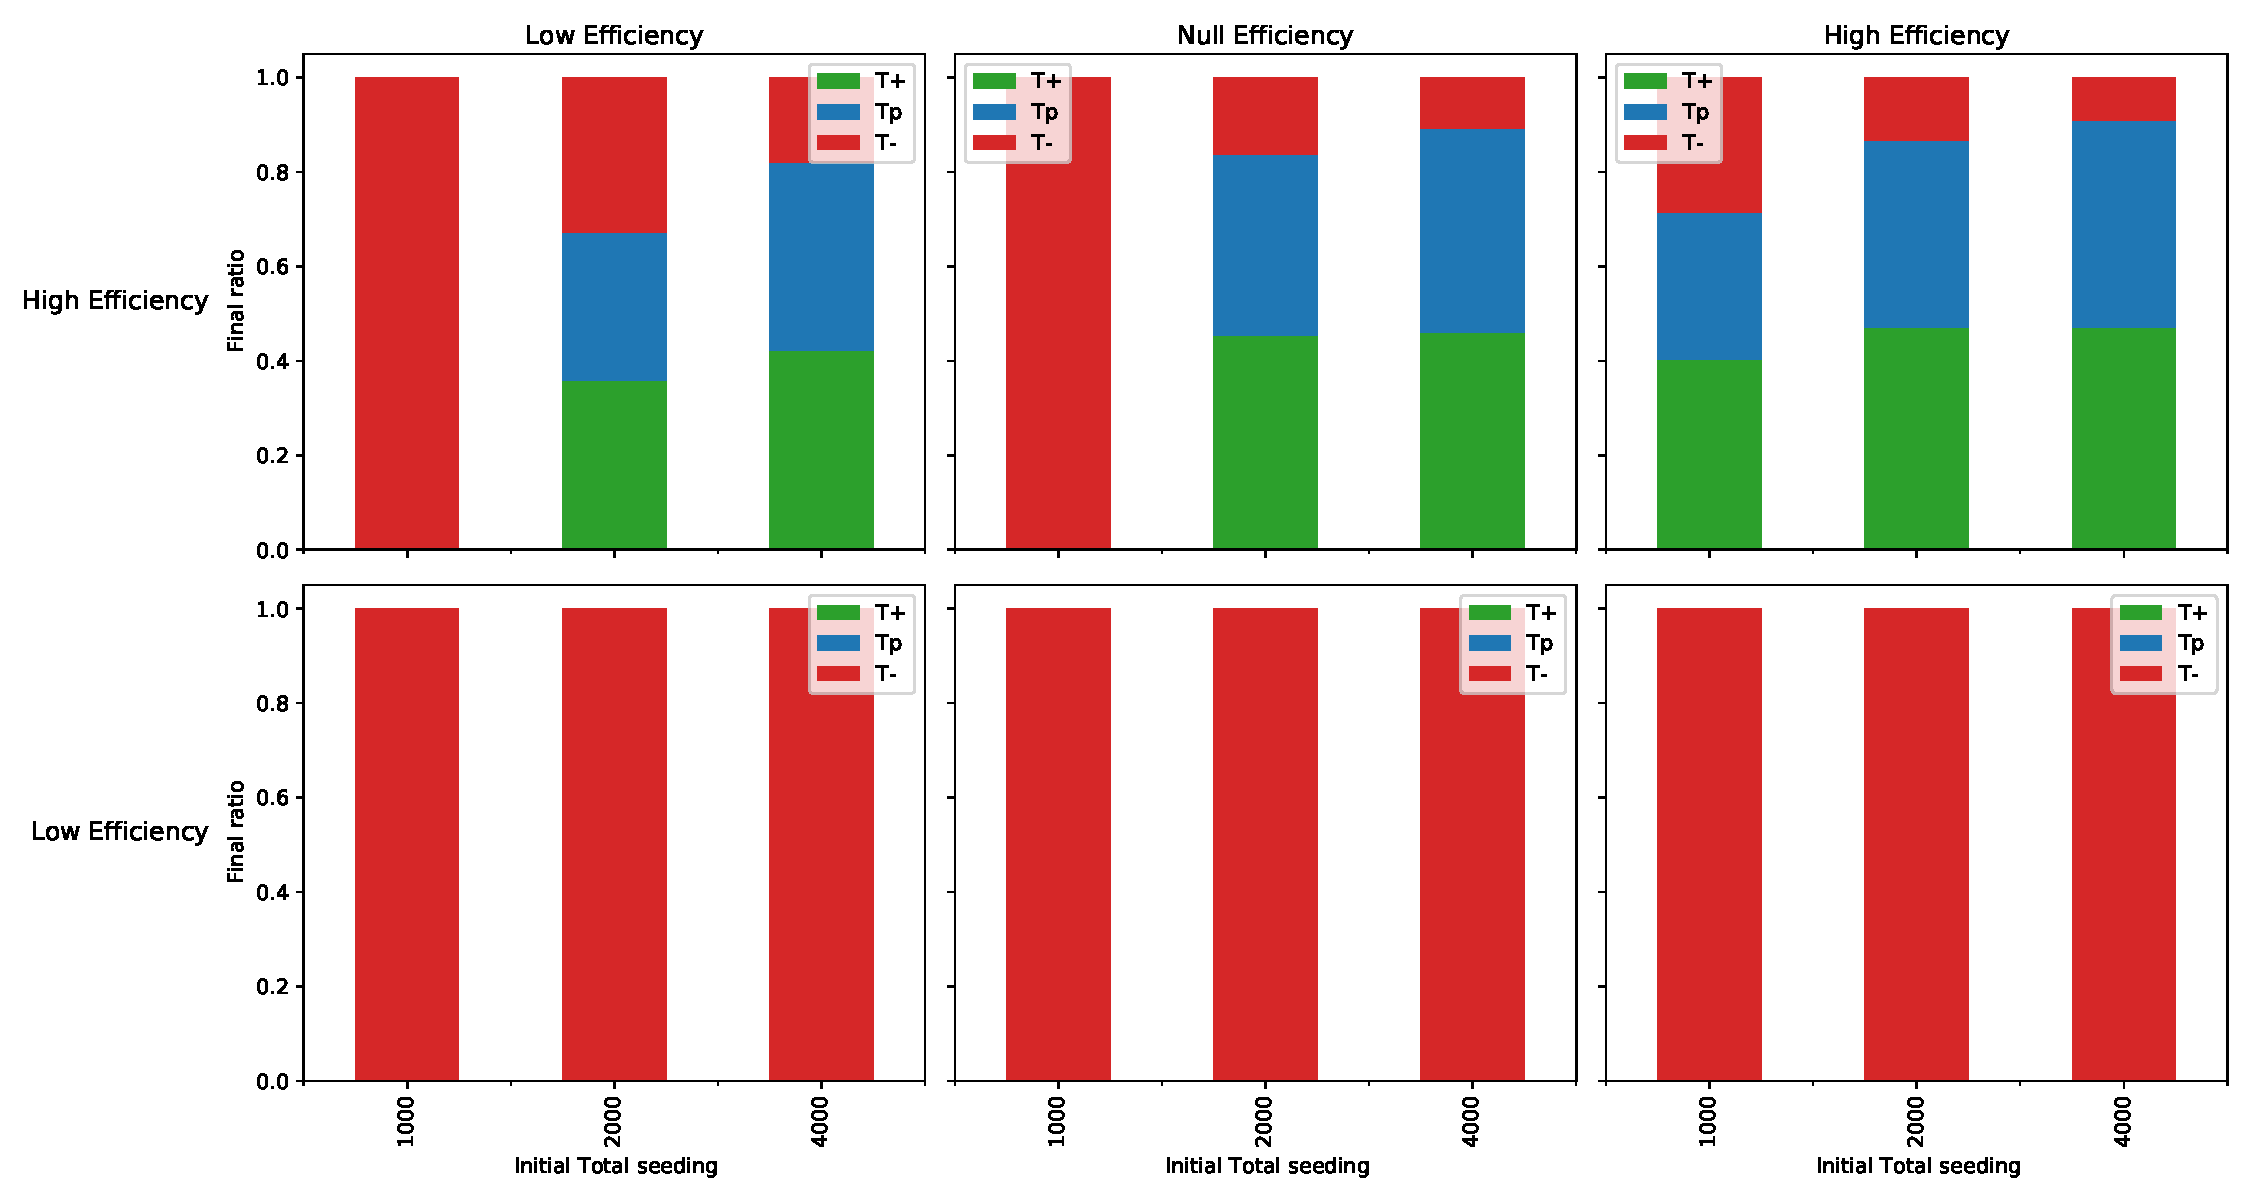
\includegraphics[width=\textwidth]{All3_efficiency_1:1:1}
        \caption{Equal seeding - 1:1:1 }
      \end{subfigure}
      \begin{subfigure}[b]{0.53\textwidth}
        \centering
        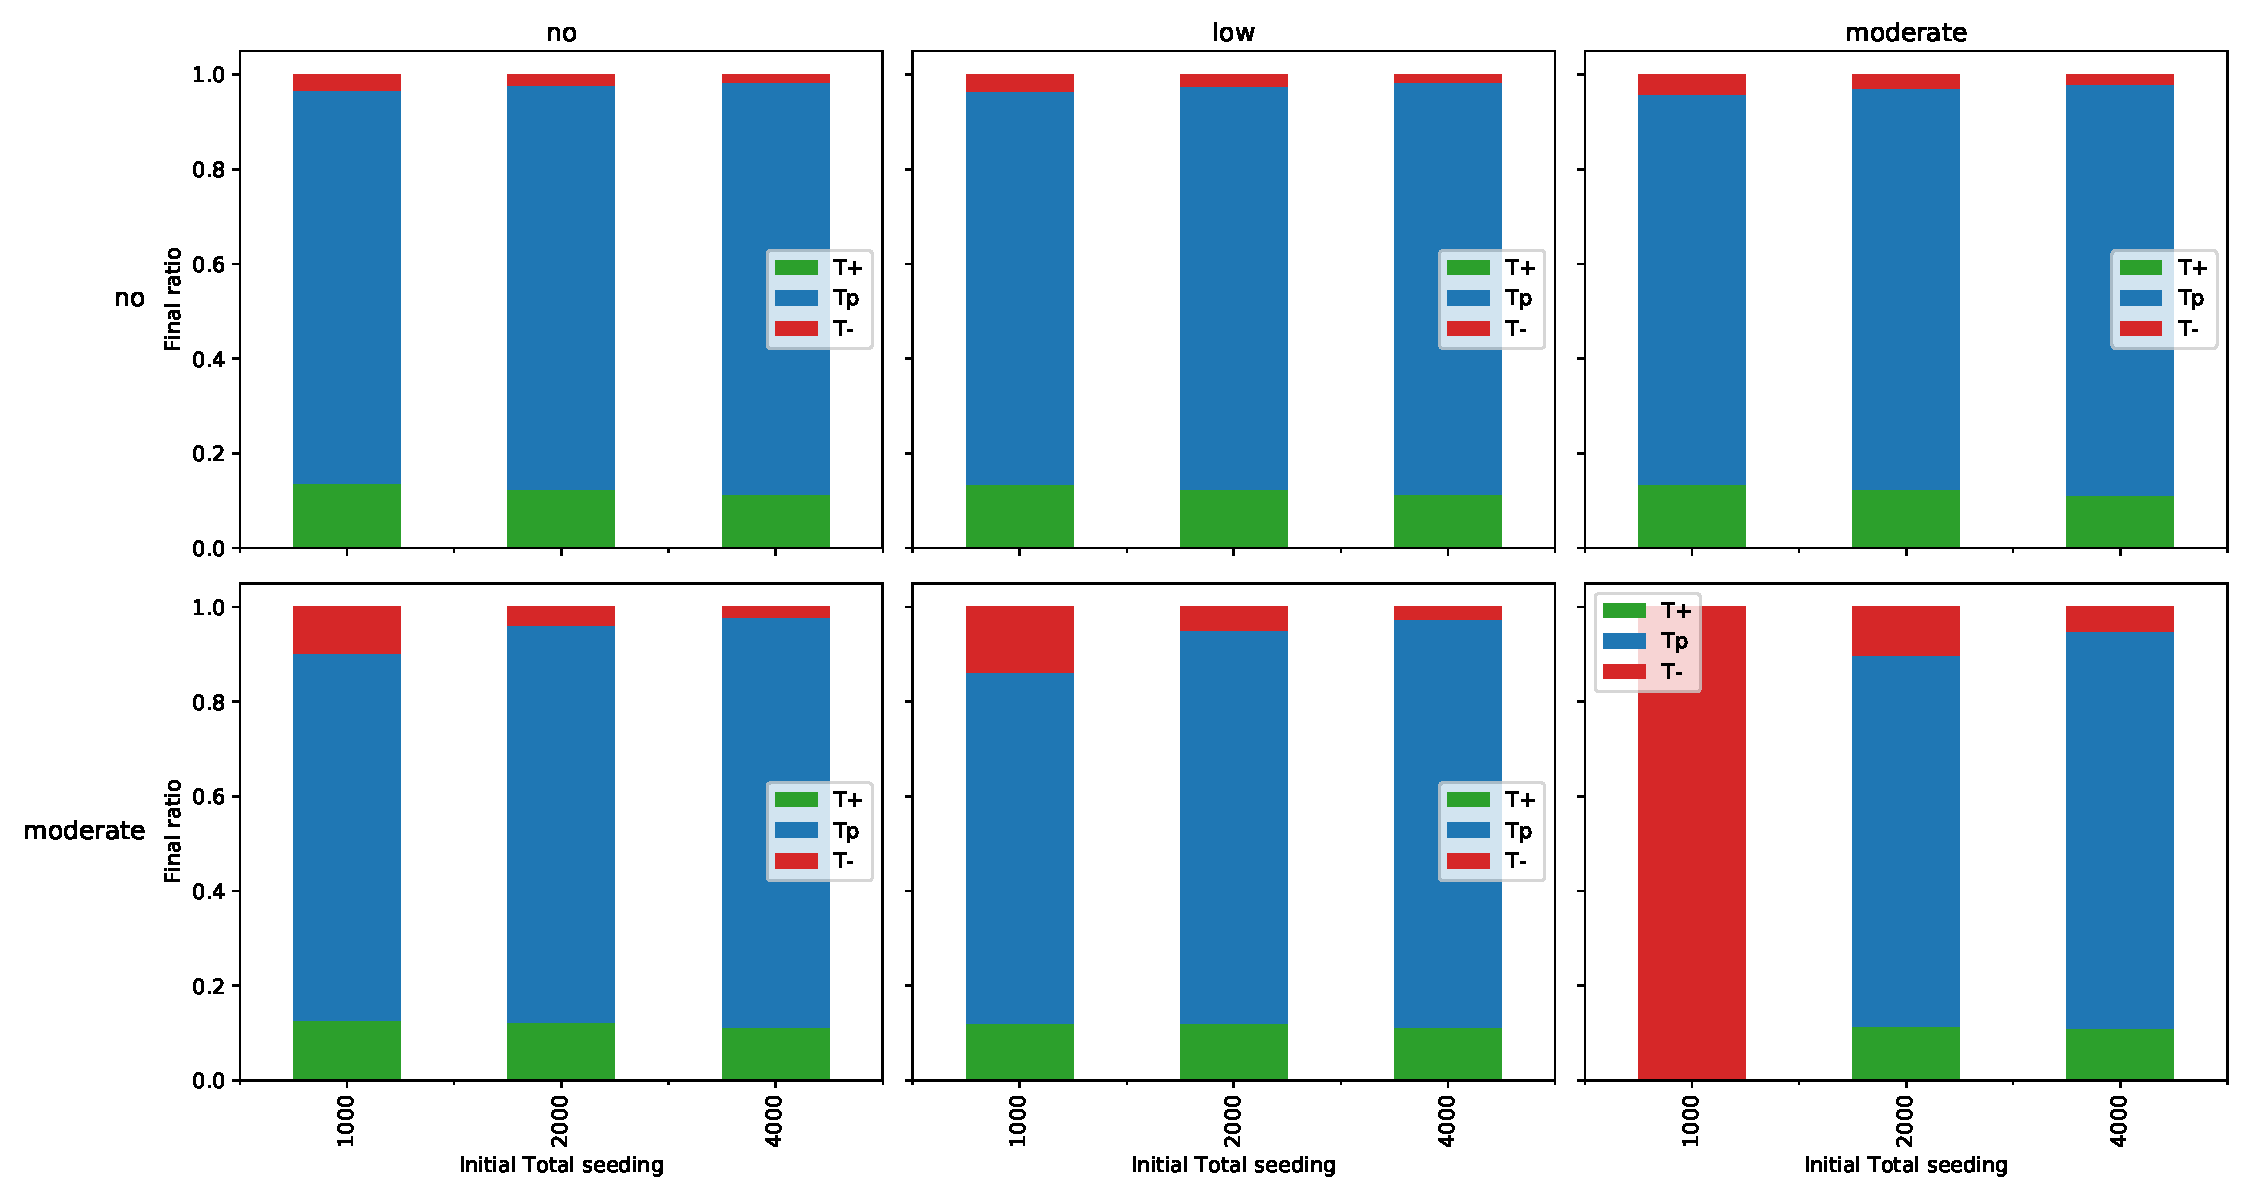
\includegraphics[width=\textwidth]{All3_efficiency_8:1:1}
        \caption{High $T^p$ seeding - 8:1:1}
      \end{subfigure}
    \end{adjustwidth}
    \caption{Final ratio of all cell types. (Stacked bar plot)}
  \end{figure}
  \begin{columns}
    \begin{column}{0.5\textwidth}
      \begin{itemize}
        \item<1-> All the cells have the same limitations
        \item<2-> Higher $T^p$ seeding ratios $\Rightarrow$ increased testosterone production
        \item<3-> Coexistence is important: tumour with $T^p$ and $T^+$ would only respond to therapy
      \end{itemize}
    \end{column}
    \begin{column}{0.5\textwidth}
      \begin{itemize}
        \item<4-> Testosterone: drastic effect on coexistence as only $T^p -T^+$ affected
        \item<5-> Oxygen: minor effect, pushes to extinction if combined limitation on the edge
      \end{itemize}
    \end{column}
  \end{columns}
\end{frame}

\section{What happens when we add therapy?}

\begin{frame}{How is it implemented?}
  \begin{columns}
    \begin{column}{0.43\textwidth}
      \begin{itemize}
        \item<1-> Therapy: modelled as boolean
        \begin{equation}
          \begin{aligned}
            & 1 = \text{MTD}\\
            & 0 = \text{no dose}
          \end{aligned}
        \end{equation}
        \item<2-> Abiraterone:
        blocks $CYP17\alpha$ \\ $T^p$, $T^+$ affected
        \begin{equation}
          p_{test}(abi) = \begin{cases}
          p_{test,max} &\text{if } abi = 0 \\
          p_{test,min} &\text{if } abi = 1 \\
          \end{cases}
          \label{p_test_dose_eq}
        \end{equation}

        \item<3-> Docetaxel: disrupts microtubule \\ All 3 affected
        \begin{equation}
          r_i(dtx) = \begin{cases}
          r_{i,max} &\text{if } dtx = 0 \\
          r_{i,min} &\text{if } dtx = 1 \\
          \end{cases}
          \label{r_dose_eq}
        \end{equation}

      \end{itemize}
    \end{column}
    \begin{column}{0.6\textwidth}
      \begin{itemize}
        \item<4-> SOC\footnotemark[1]: dose given at MTD\footnotemark[1] from the beginning
        \begin{equation}
          dose(y,t) = 1 \quad \forall\ t, y
          \label{dose_soc_eq}
        \end{equation}
        \item<5-> AT\footnotemark[1]: binary mode considered
        \begin{itemize}
          \item Dose at MTD\footnotemark[1] when on
          \item Therapy turned on when population above On threshold
          \item Therapy turned off when population below Off threshold
        \end{itemize}
        \begin{equation}
          dose(y,t) = \begin{cases}
          0 &\text{if } dose(y,t-\Delta t) = 0 \text{ and } y < \text{On} \\
          1 &\text{if } dose(y,t-\Delta t) = 0 \text{ and } y \geq \text{On} \\
          1 &\text{if } dose(y,t-\Delta t) = 1 \text{ and } y > \text{Off} \\
          0 &\text{if } dose(y,t-\Delta t) = 1 \text{ and } y \leq \text{Off} \\
          \end{cases}
          \label{dose_at_eq}
        \end{equation}
      \end{itemize}
    \end{column}
  \end{columns}
  \footnotetext[1]{MTD: Maximum tolerated dose, SOC: Standard-Of-Care, AT: Adaptive Therapy}
  \footnotetext[2]{abi: abiraterone, dtx: docetaxel}
\end{frame}

\begin{frame}{What happens with Standard-Of-Care?}
  \begin{figure}[h]
    \begin{adjustwidth}{-5cm}{-5cm}
      \centering
      \begin{subfigure}[b]{0.53\textwidth}
        \centering
        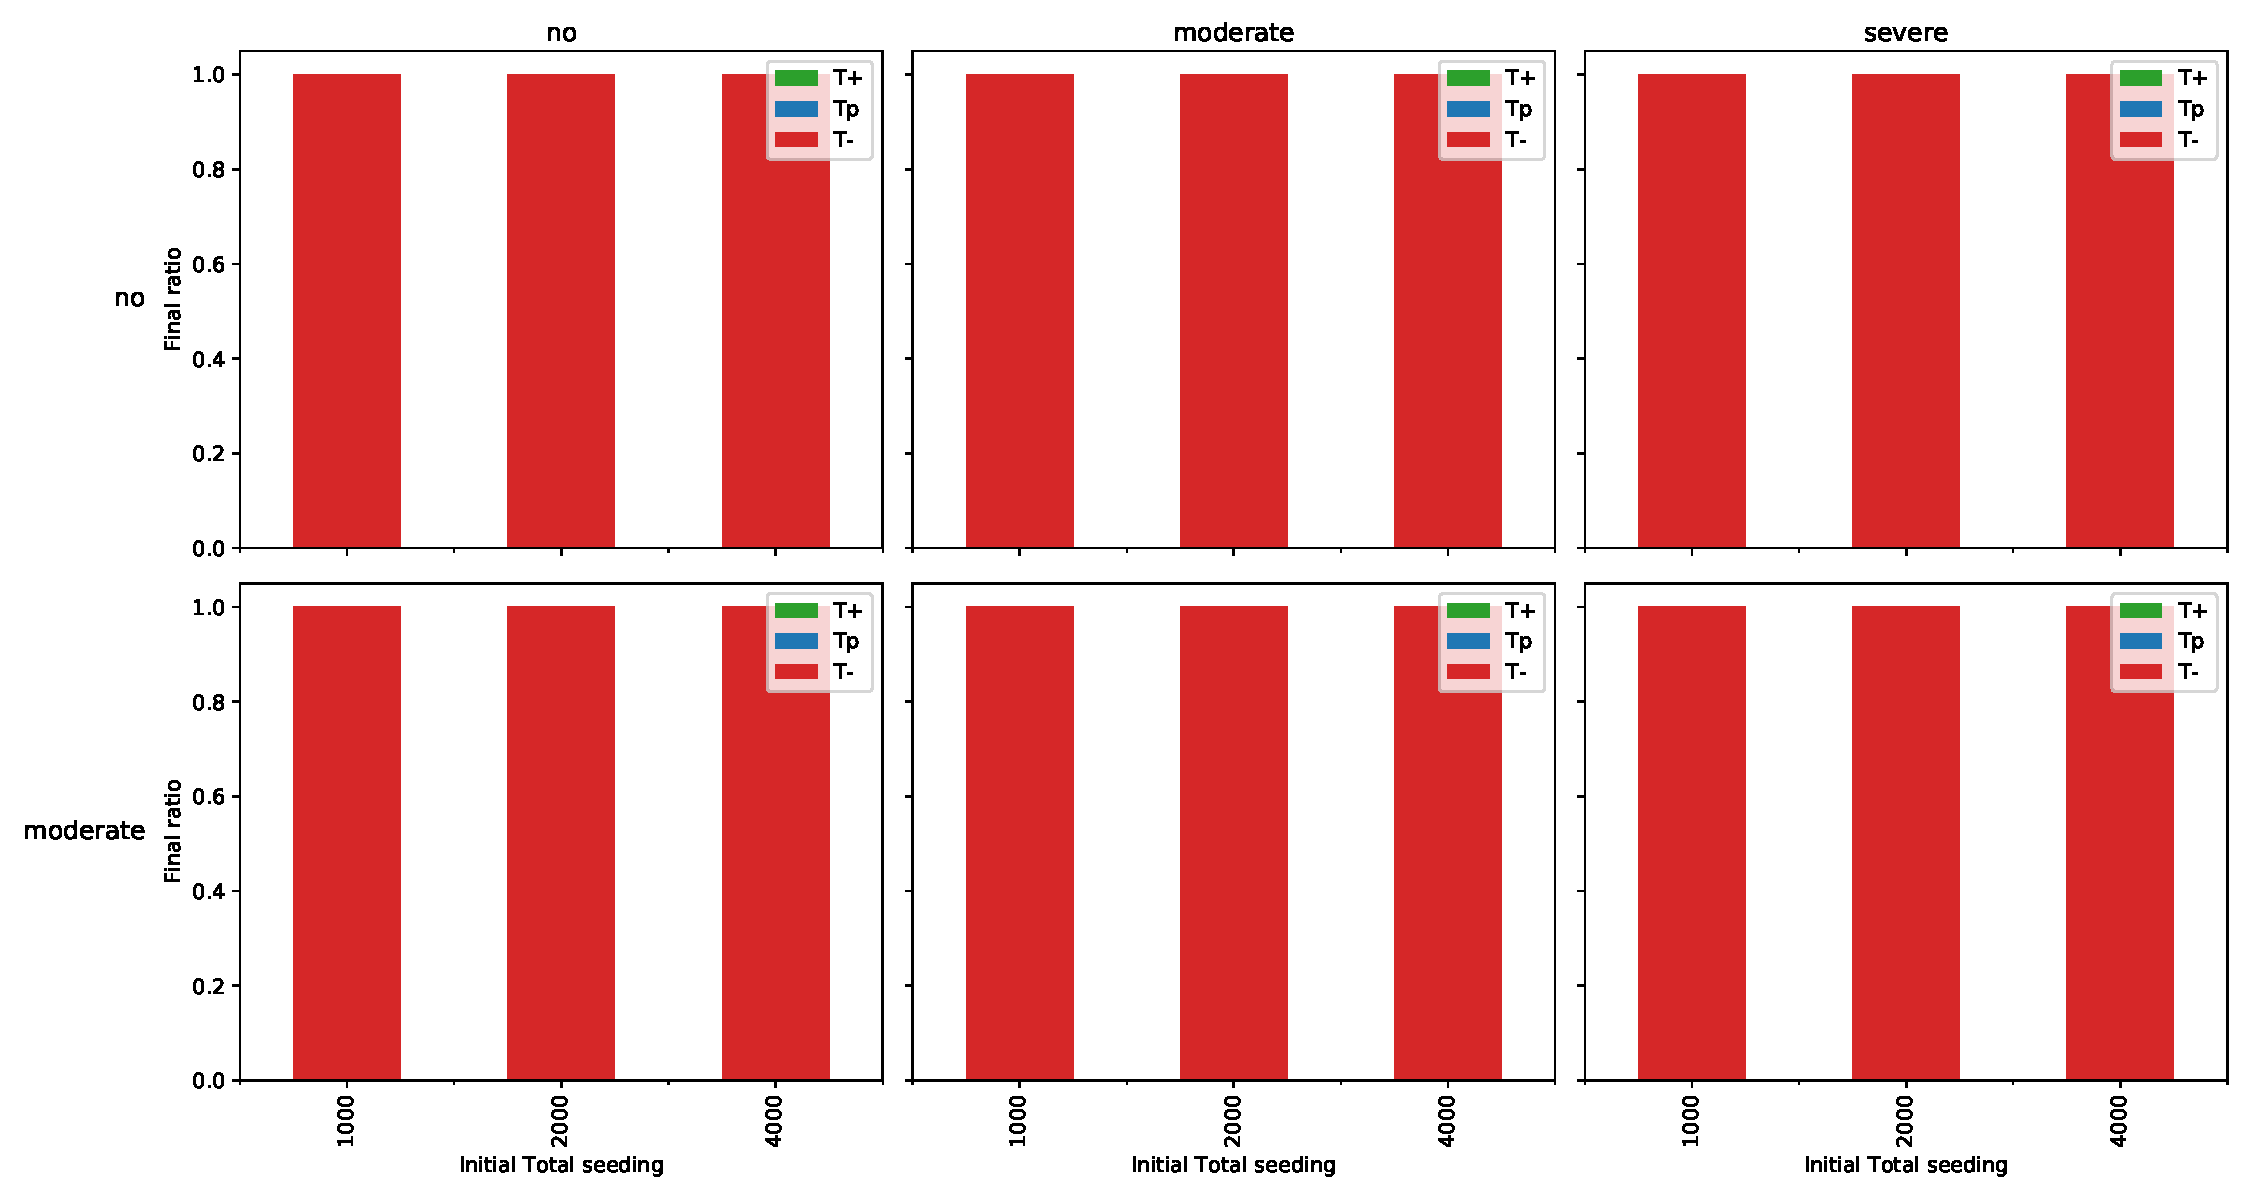
\includegraphics[width=\textwidth]{All3_therapy-SOC_1:1:1}
        \caption{Equal seeding - 1:1:1}
      \end{subfigure}
      \begin{subfigure}[b]{0.53\textwidth}
        \centering
        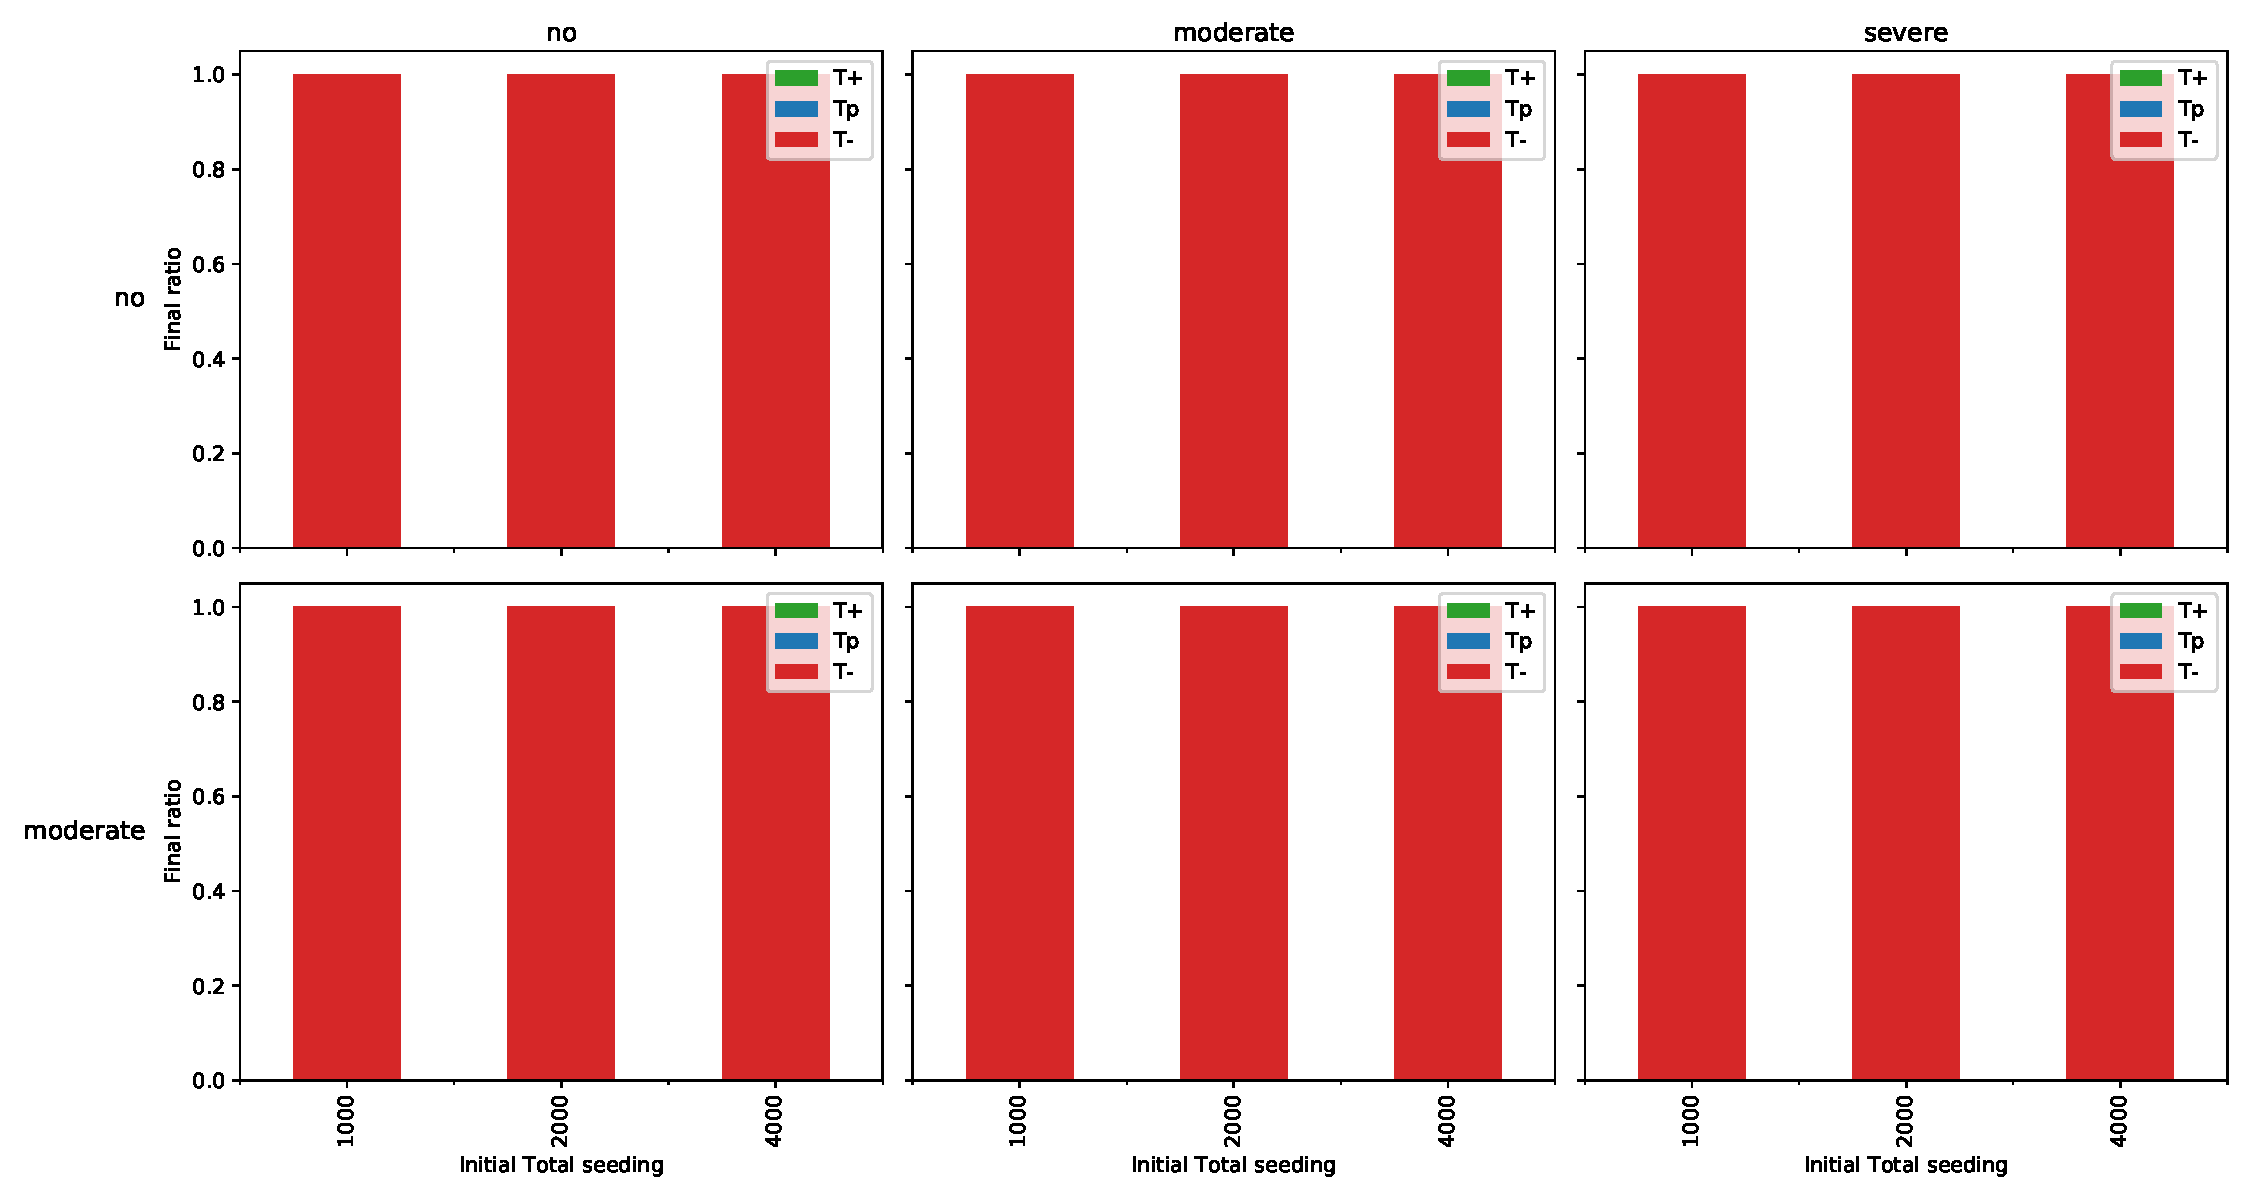
\includegraphics[width=\textwidth]{All3_therapy-SOC_8:1:1}
        \caption{High $T^p$ seeding - 8:1:1}
      \end{subfigure}
    \end{adjustwidth}
    \caption{Final ratio of all cell types under standard-of-care. (Stacked bar plot)}
  \end{figure}
  \begin{columns}
    \begin{column}{0.5\textwidth}
      \begin{itemize}
        \item $T^+, T^p$ go extinct in all cases
      \end{itemize}
    \end{column}
    \begin{column}{0.5\textwidth}
      \begin{itemize}
        \item Testosterone levels insufficient for growth
      \end{itemize}
    \end{column}
  \end{columns}
\end{frame}

\begin{frame}{Thresholds for Adaptive Therapy }
  \begin{figure}[h]
    \centering
    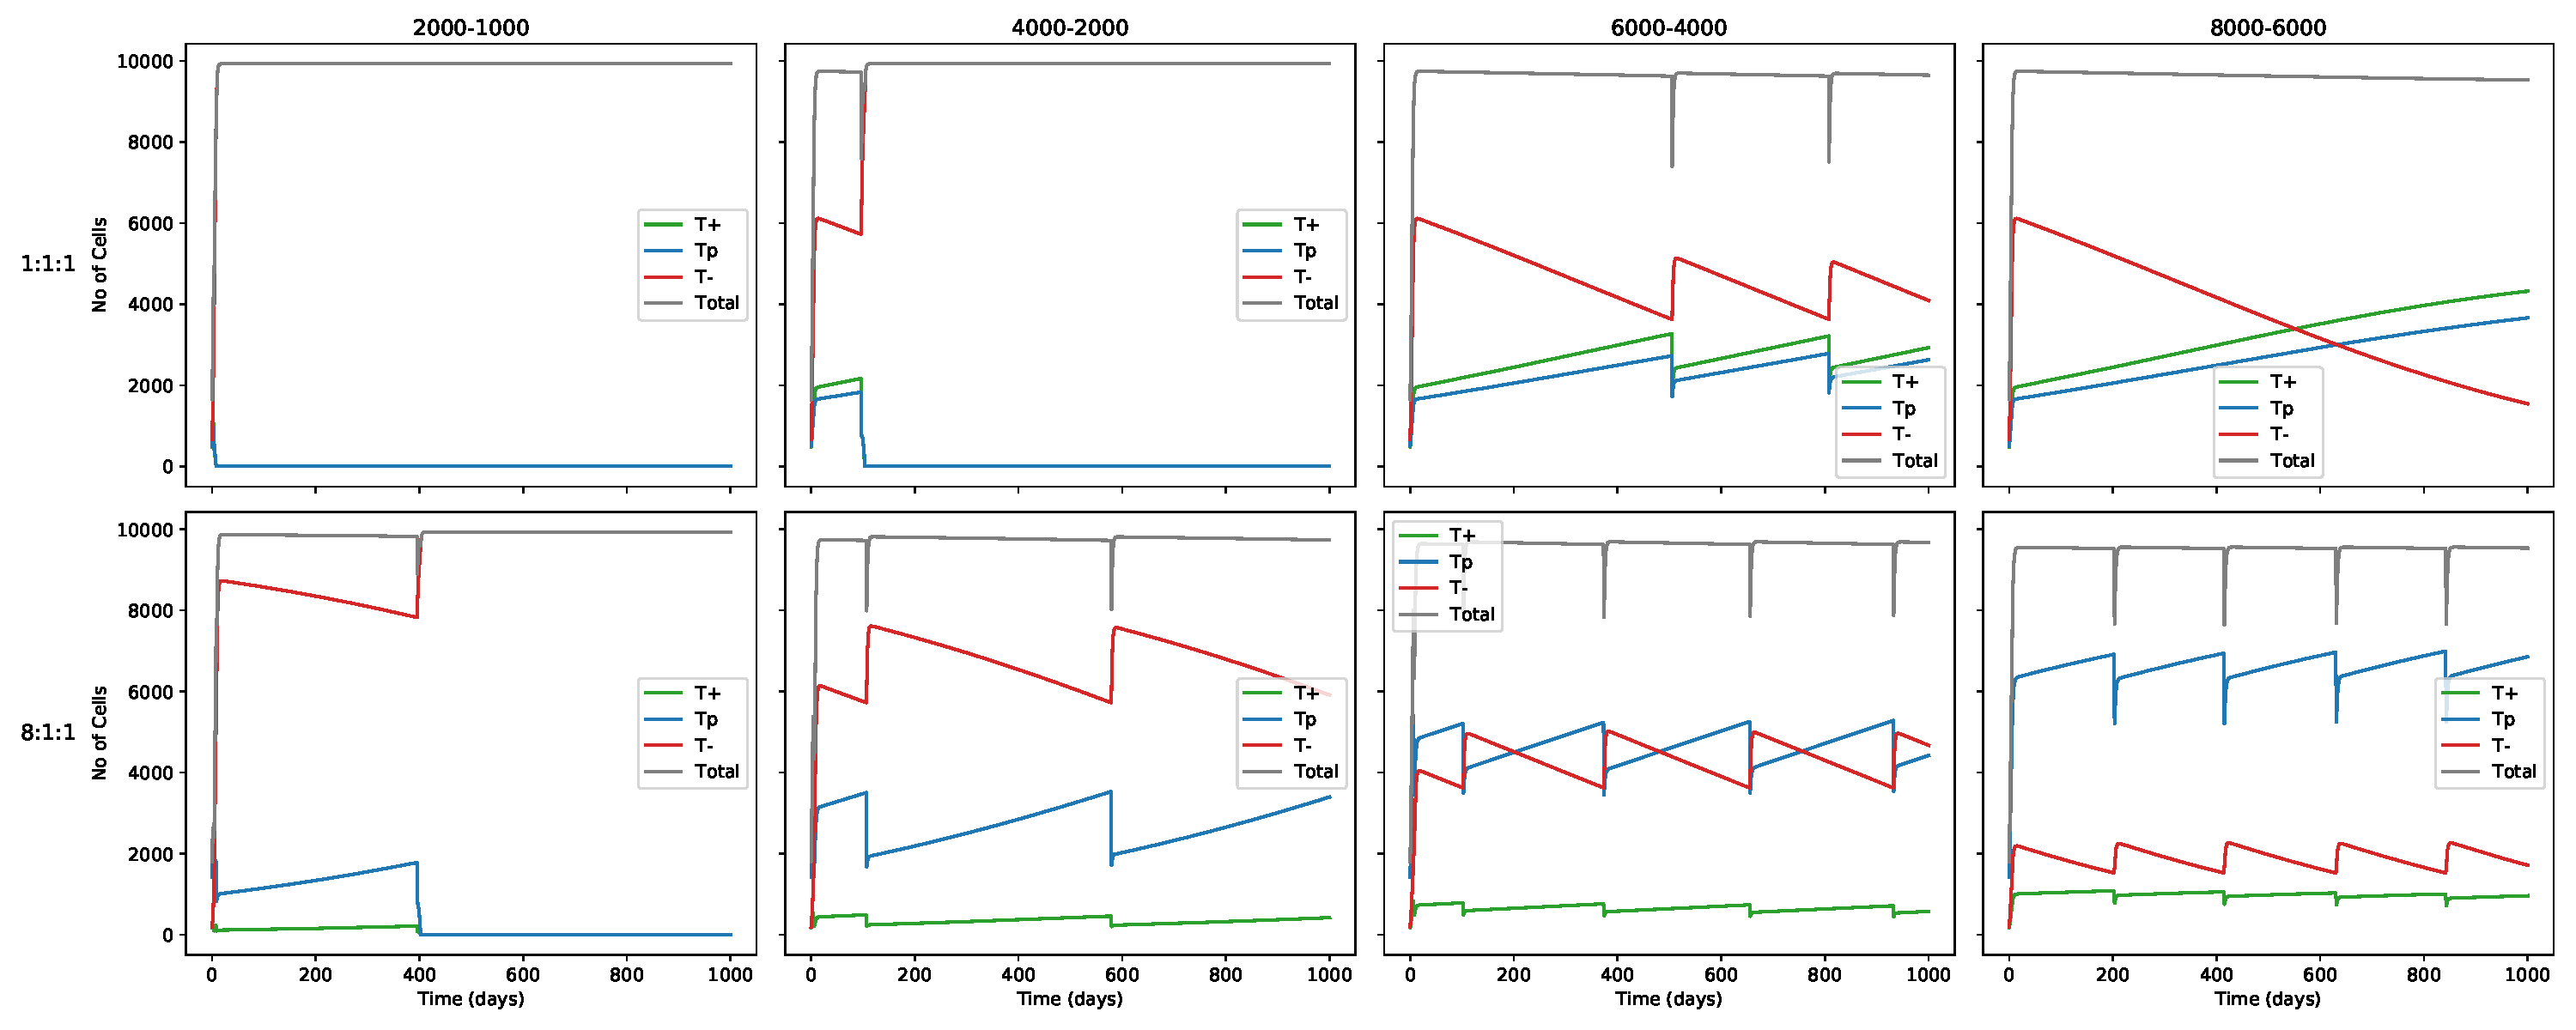
\includegraphics[width=0.7\textwidth]{All3_therapy-standardization}
    \caption{Standardisation of threshold for adaptive therapy}
  \end{figure}
  \begin{columns}
    \begin{column}{0.65\textwidth}
      \begin{itemize}
        \item<1-> Low threshold: $T^-$ inhibits $T^p - T^+$ and causes extinction
        \item<2-> High threshold: $T^+ - T^p$ can compete with $T^-$ \cite{Hansen}
        \item<3-> Too High: No therapy applied as On threshold never crossed
        \item<4-> Chosen- On: 6000, Off: 4000
      \end{itemize}
    \end{column}
    \begin{column}{0.4\textwidth}
      \begin{itemize}
        \item<5-> $T^+ + T^p$ only for threshold
        \item<5-> With total: $T^+ - T^p$ go extinct before therapy turned off
      \end{itemize}
    \end{column}
  \end{columns}
\end{frame}

\begin{frame}{Is Adaptive Therapy better?}
  \begin{figure}[h]
    \begin{adjustwidth}{-5cm}{-5cm}
      \centering
      \begin{subfigure}[b]{0.53\textwidth}
        \centering
        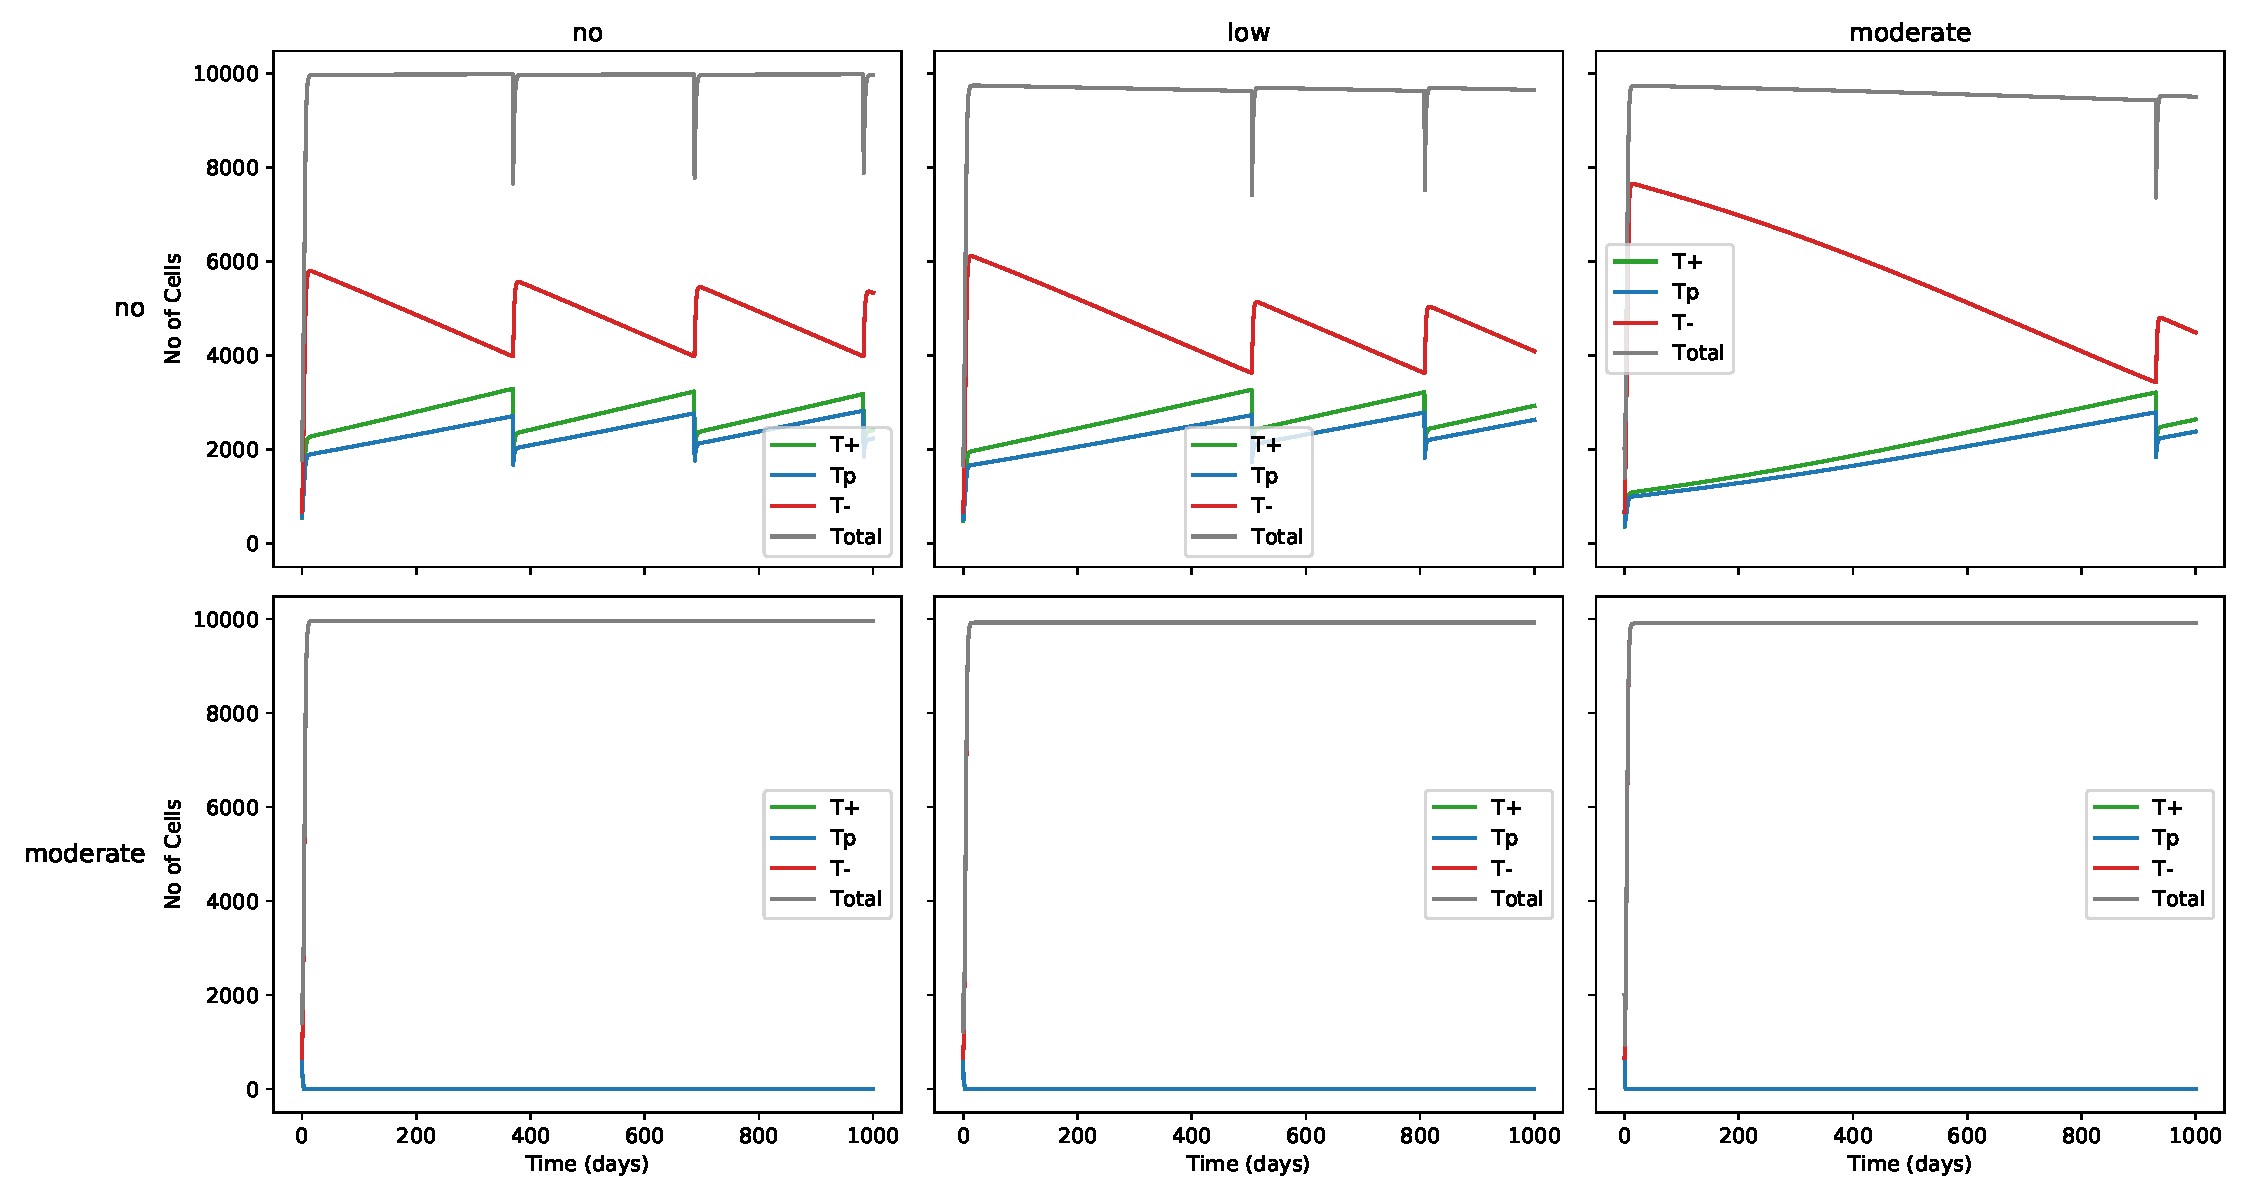
\includegraphics[width=\textwidth]{All3_therapy_1:1:1-2000}
        \caption{Equal seeding - 1:1:1}
      \end{subfigure}
      \begin{subfigure}[b]{0.53\textwidth}
        \centering
        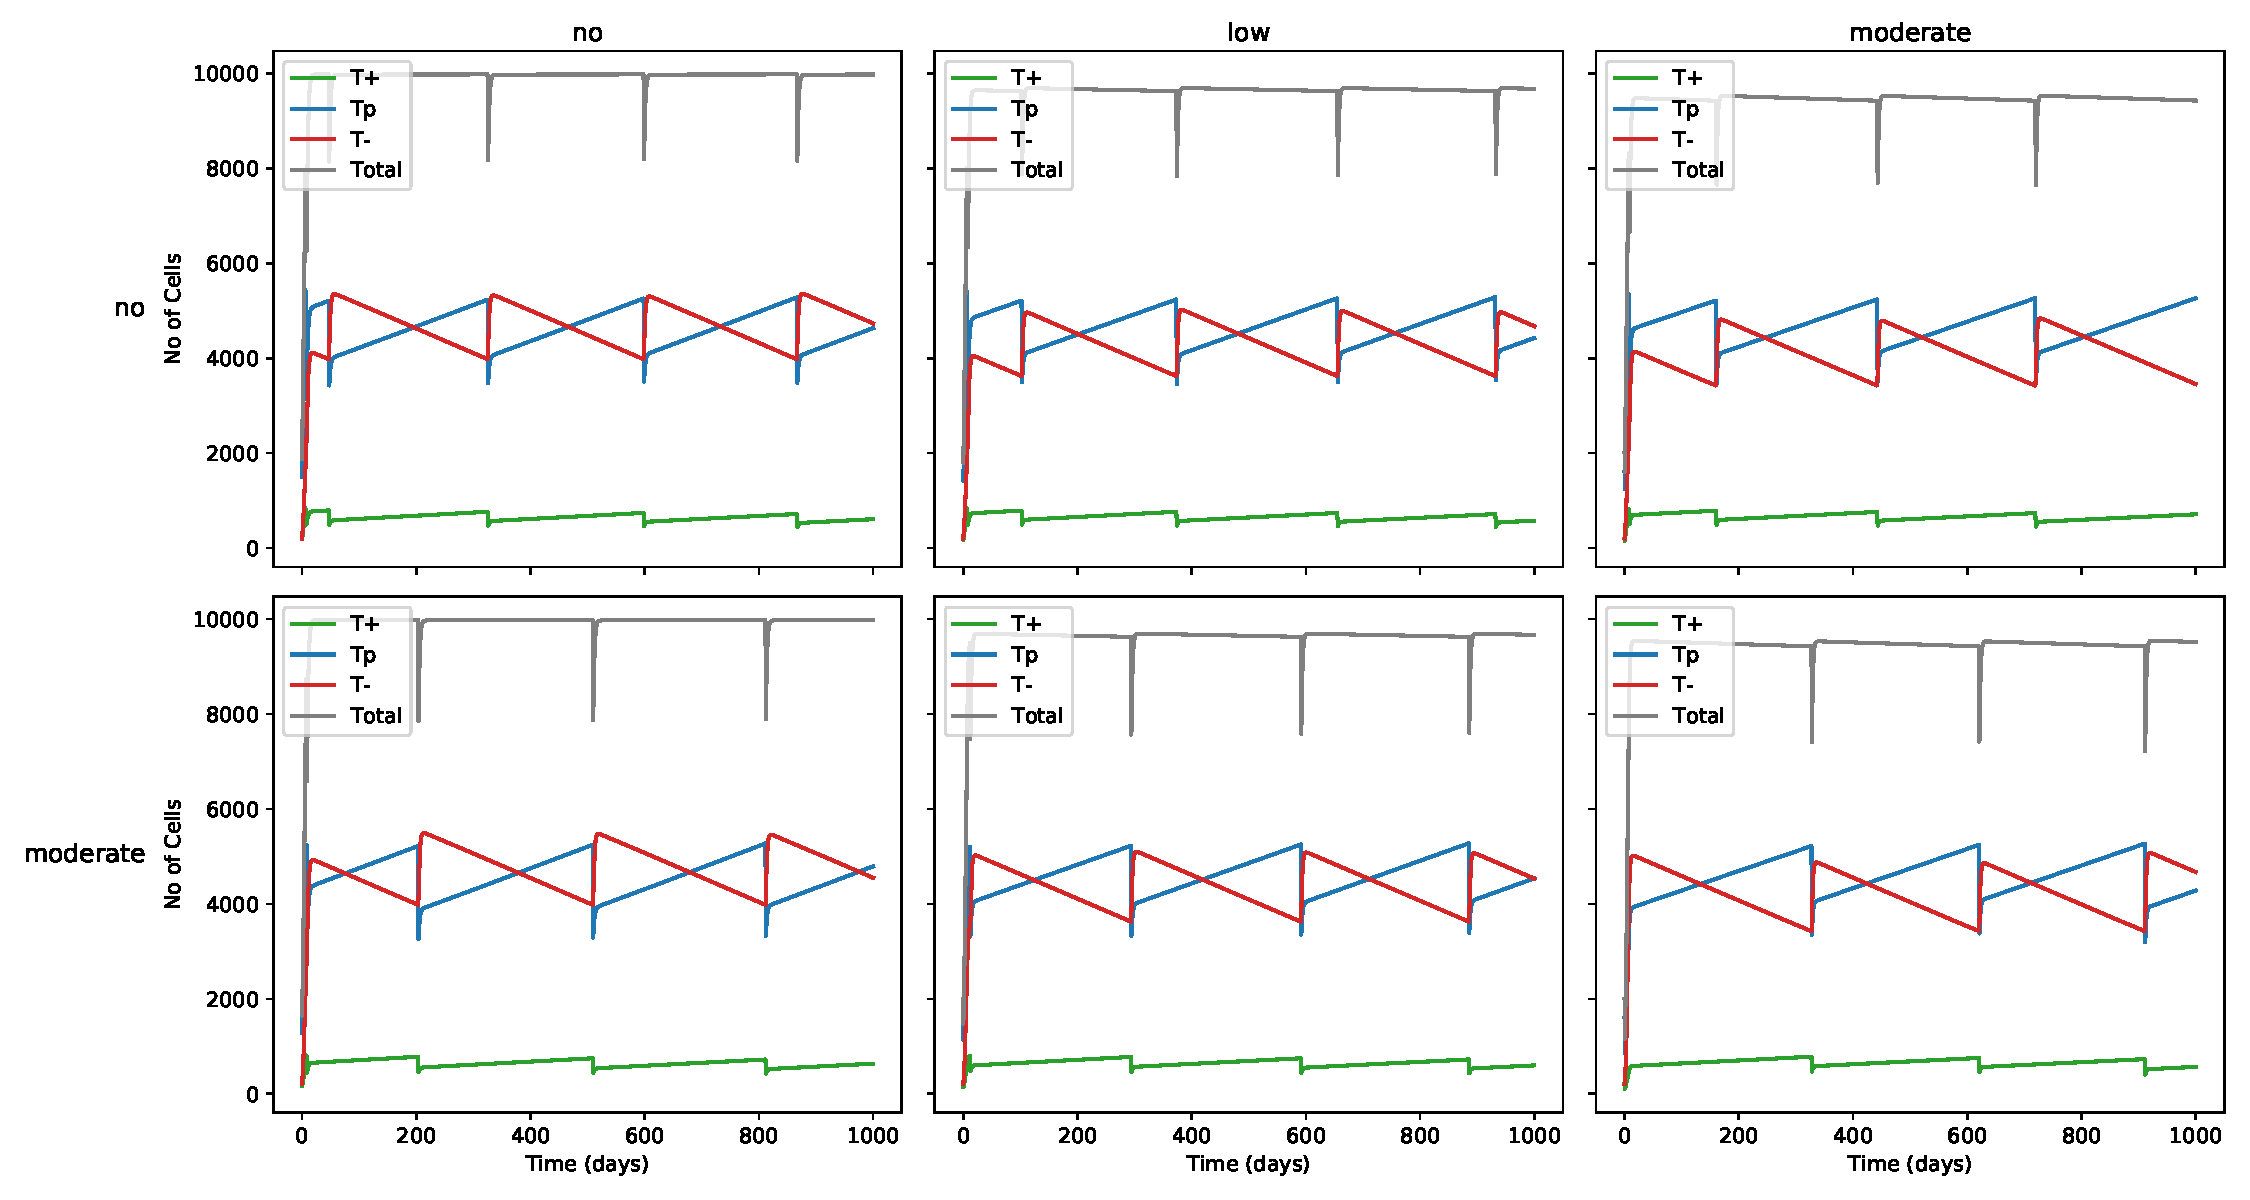
\includegraphics[width=\textwidth]{All3_therapy_8:1:1-2000}
        \caption{High $T^p$ seeding - 8:1:1}
      \end{subfigure}
    \end{adjustwidth}
    \caption{Time-series of all cell types with adaptive therapy. (On:6000, Off:4000)}
  \end{figure}
  \begin{columns}
    \begin{column}{0.5\textwidth}
      \begin{itemize}
        \item<1-> $T^+ - T^p$ extinct just by competition: no effect
        \item<2-> More $T^+ - T^p$ $\rightarrow$ more responsive to abiraterone and better suppress $T^-$
      \end{itemize}
    \end{column}
    \begin{column}{0.5\textwidth}
      \begin{itemize}
        \item<3-> Success of Adaptive therapy:
        \begin{itemize}
          \item<4-> $\checkmark$ Preventing competitive release of resistant
          \item<5-> $\times$ Reducing tumour burden: $T^-$ replace dead cells
        \end{itemize}
      \end{itemize}
    \end{column}
  \end{columns}
\end{frame}

\section{Can adaptive therapy be even made better?}

\begin{frame}{Can delaying treatment help?}
  \begin{figure}[h]
    \begin{adjustwidth}{-5cm}{-5cm}
      \centering
      \begin{subfigure}[b]{0.53\textwidth}
        \centering
        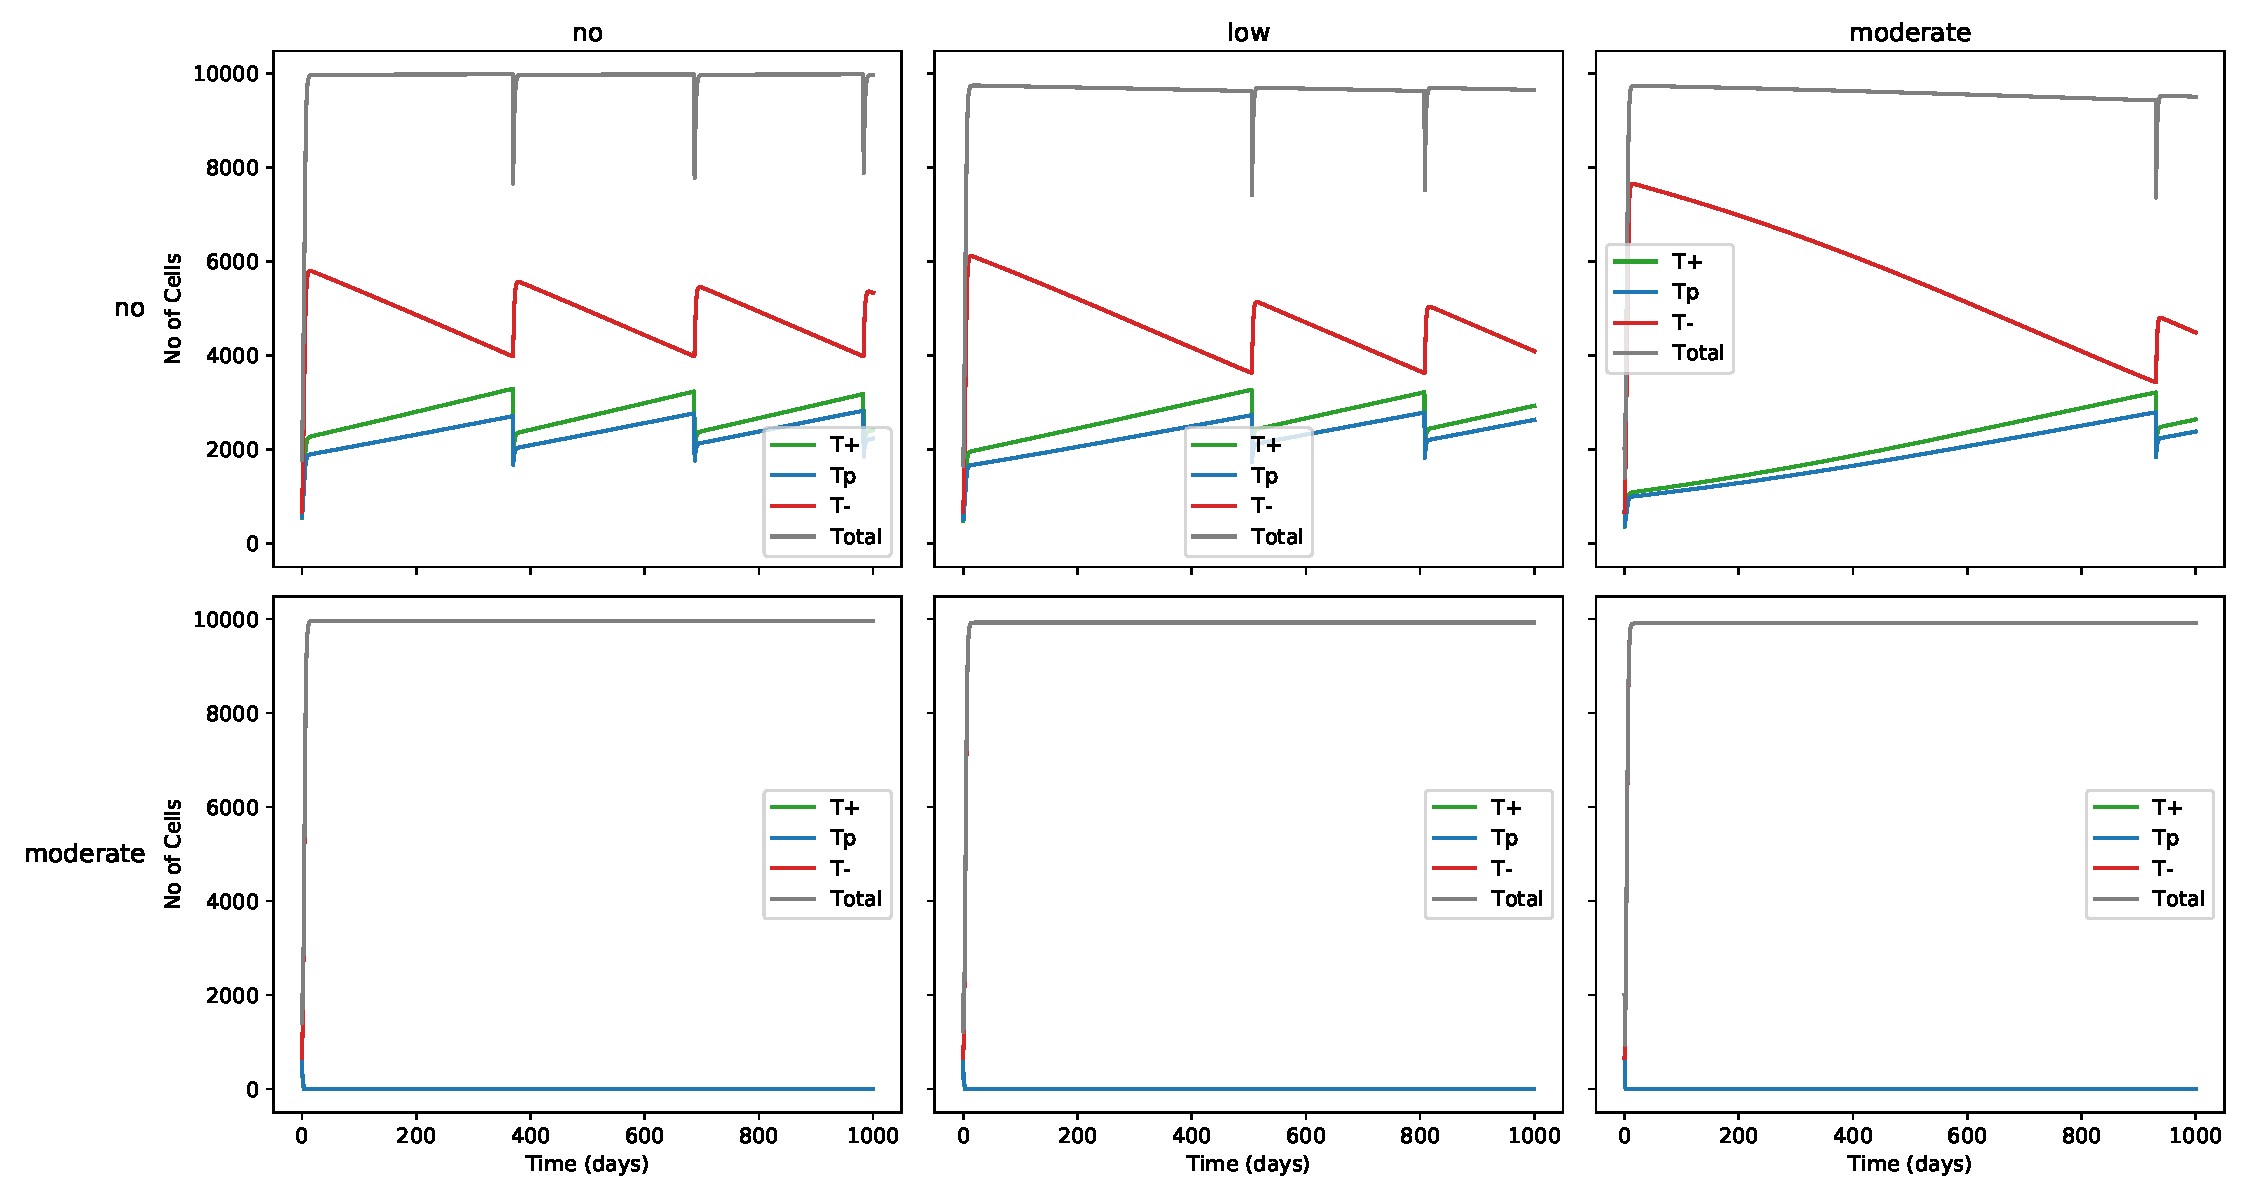
\includegraphics[width=\textwidth]{All3_therapy_200day_1:1:1}
        \caption{Equal seeding - 1:1:1}
      \end{subfigure}
      \begin{subfigure}[b]{0.53\textwidth}
        \centering
        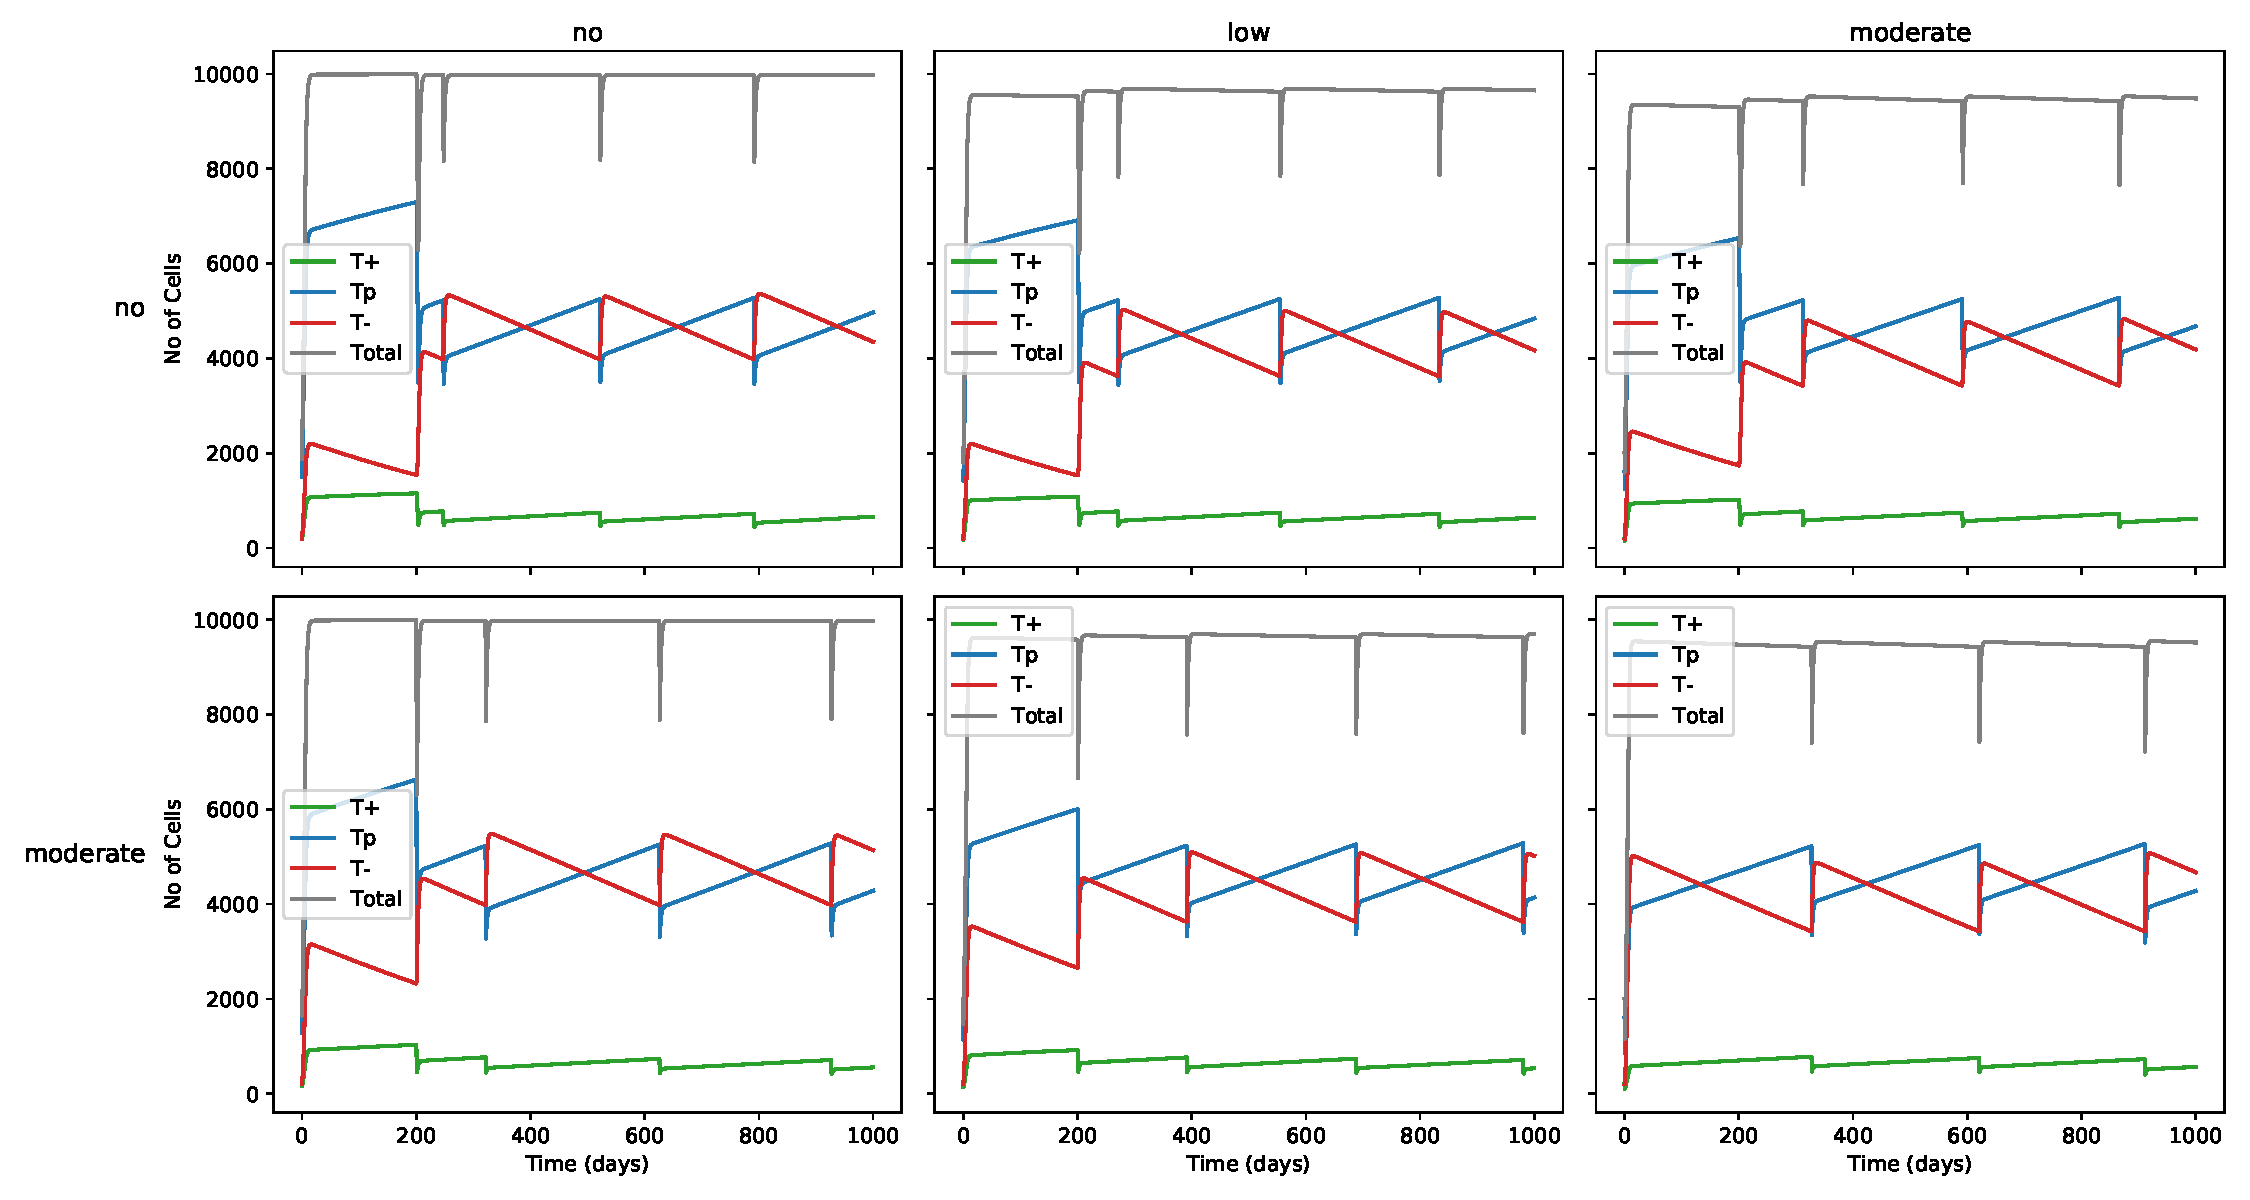
\includegraphics[width=\textwidth]{All3_therapy_200day_8:1:1}
        \caption{High $T^p$ seeding - 8:1:1}
      \end{subfigure}
    \end{adjustwidth}
    \caption{Time-series of all cell types with adaptive therapy delayed by 200 days. (On:6000, Off:4000)}
  \end{figure}
  \begin{columns}
    \begin{column}{0.5\textwidth}
      \begin{itemize}
        \item<1-> $T^+ - T^p$ $\uparrow$ in periods of no therapy
        \item<2-> Speculation: Can delaying bring better balance between $T^+ - T^p$ and $T^-$?
      \end{itemize}
    \end{column}
    \begin{column}{0.5\textwidth}
      \begin{itemize}
        \item<3-> No advantage found as they have similar temporal dynamics
      \end{itemize}
    \end{column}
  \end{columns}
\end{frame}

\begin{frame}{What about using multiple drugs?}
  \begin{figure}[h]
    \begin{adjustwidth}{-5cm}{-5cm}
      \centering
      \begin{subfigure}[b]{0.53\textwidth}
        \centering
        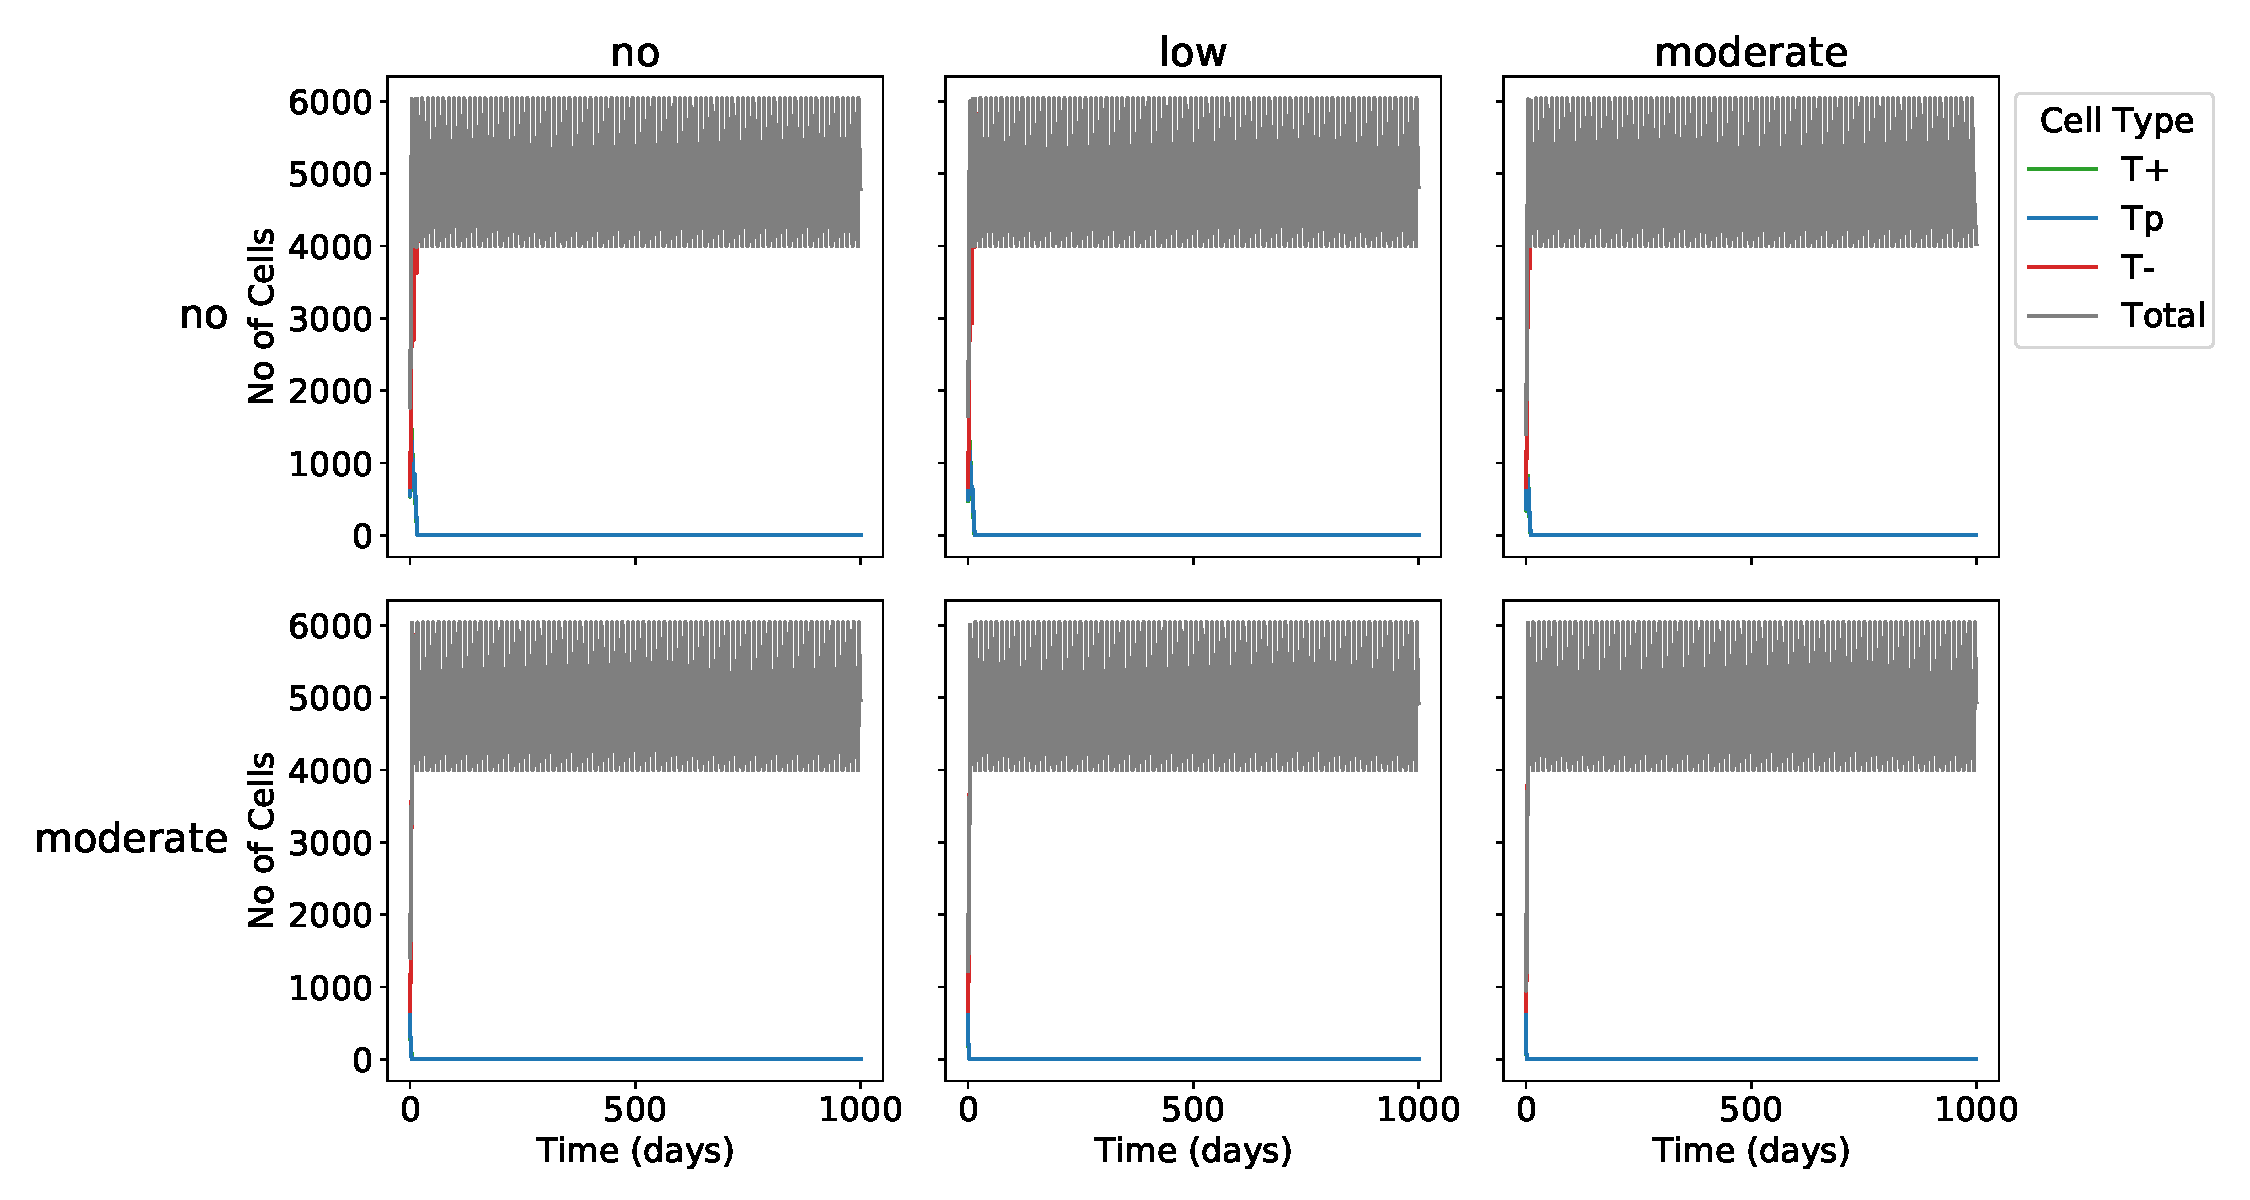
\includegraphics[width=\textwidth]{All3_therapy-combi_1:1:1}
        \caption{Equal seeding - 1:1:1}
      \end{subfigure}
      \begin{subfigure}[b]{0.53\textwidth}
        \centering
        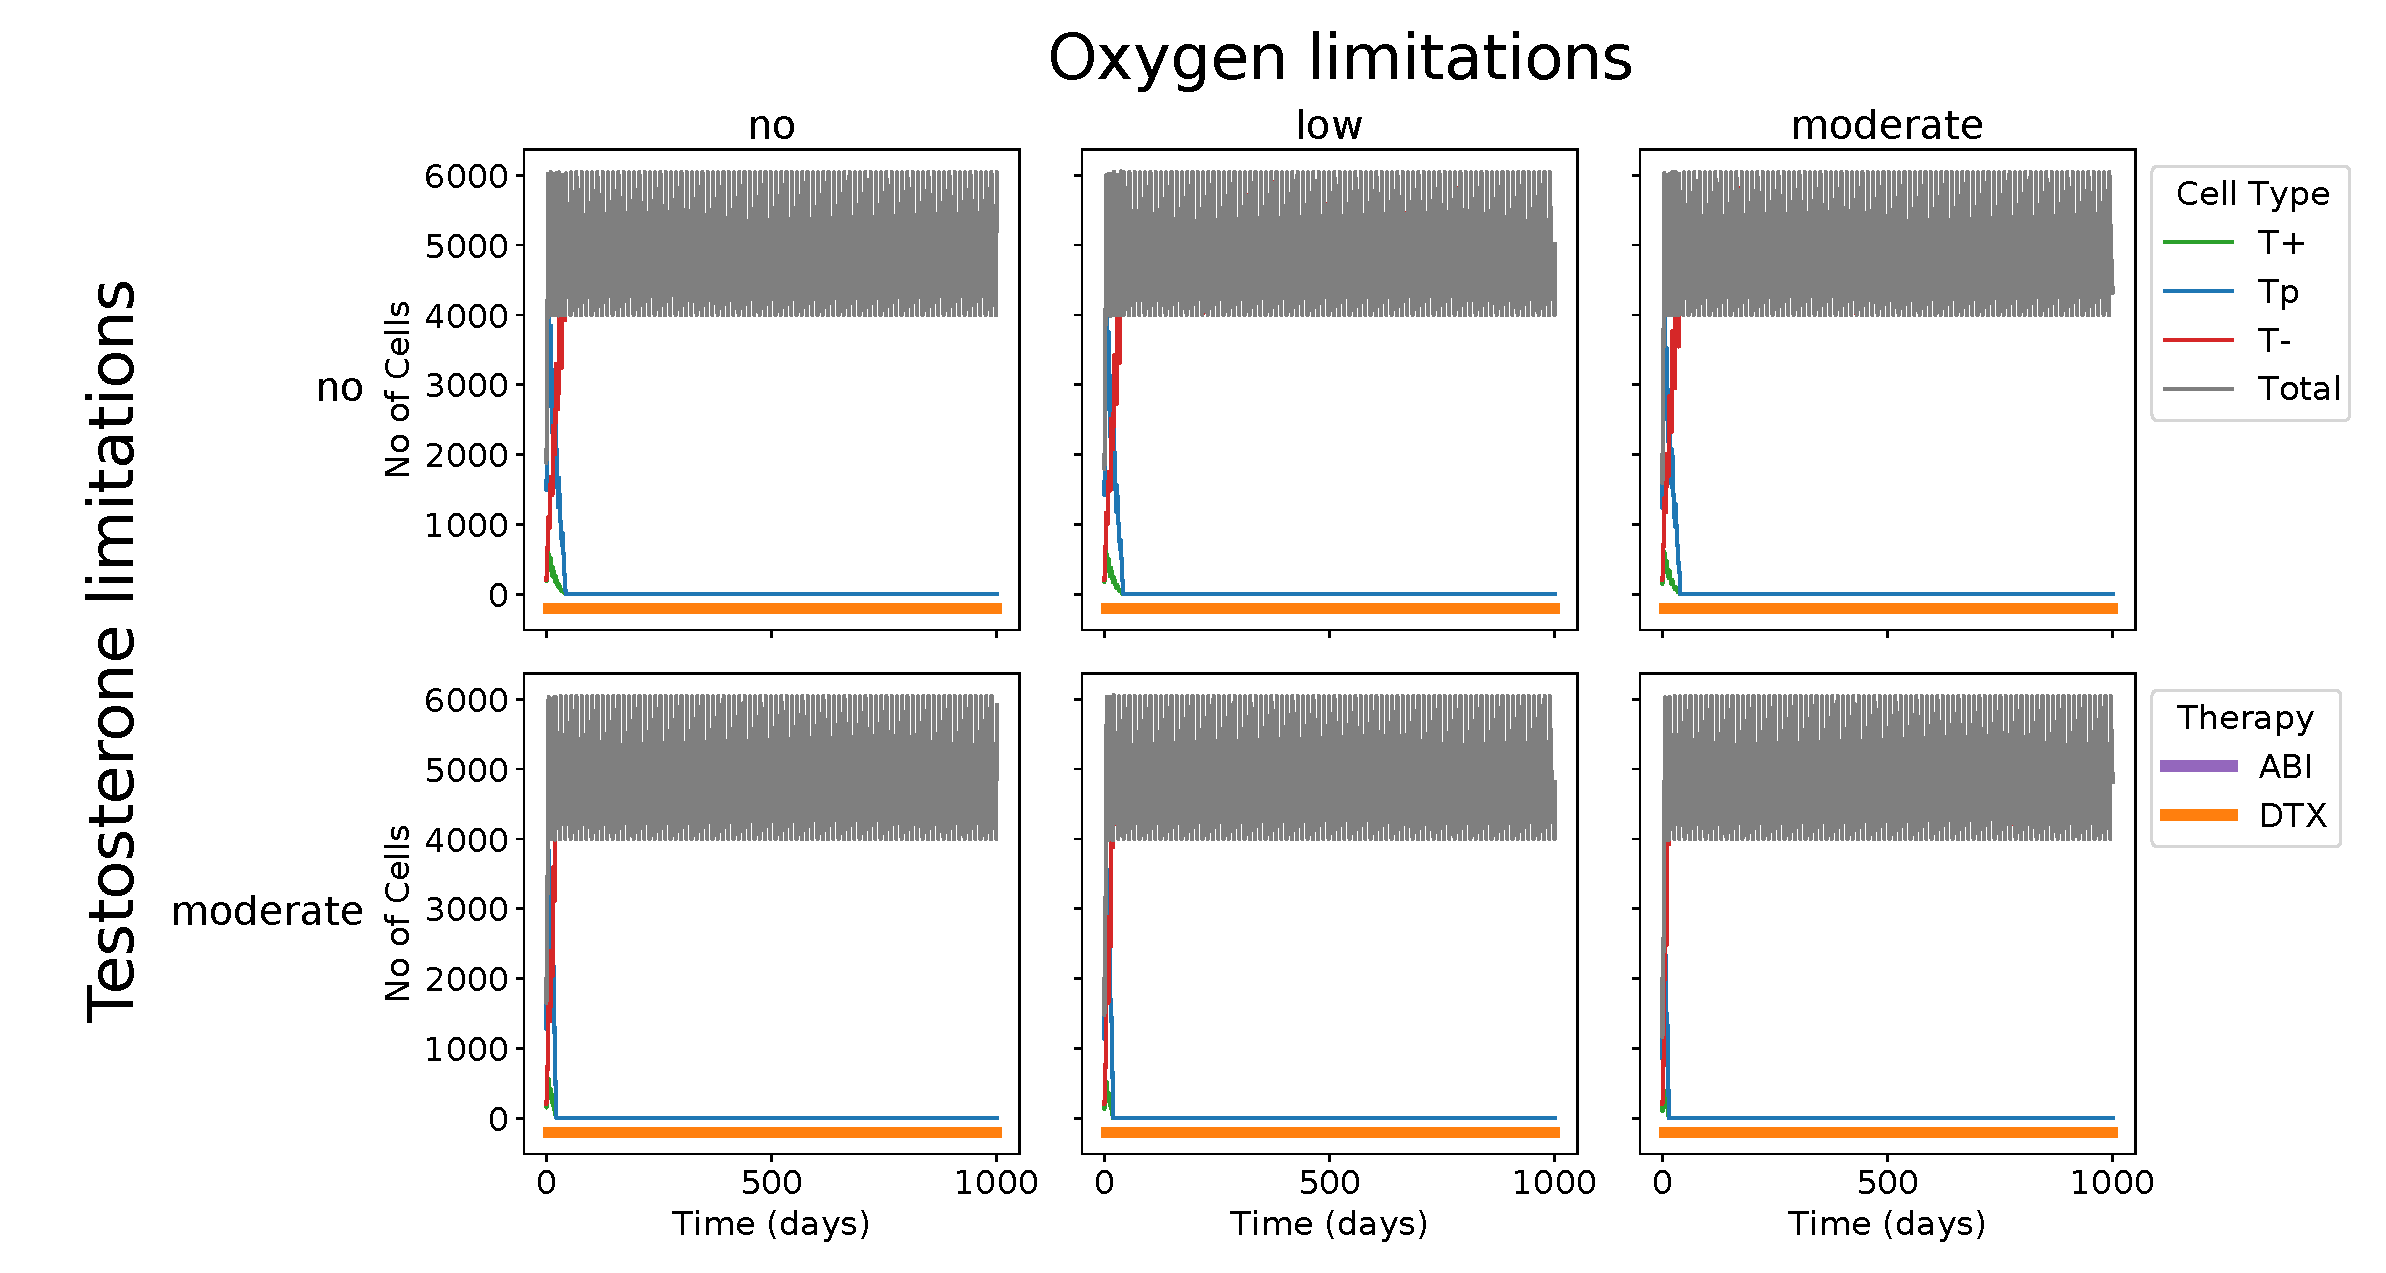
\includegraphics[width=\textwidth]{All3_therapy-combi_8:1:1}
        \caption{High $T^p$ seeding - 8:1:1}
      \end{subfigure}
    \end{adjustwidth}
    \caption{Time-series of all cell types with combination adaptive therapy of abi and dtx\footnotemark[1]. abi(On:6000, Off:4000; $T^+ + T^p$), dtx(On:6000, Off:4000; Total)}
  \end{figure}
  \begin{columns}
    \begin{column}{0.5\textwidth}
      \begin{itemize}
        \item<1-> Hormonal (abi\footnotemark[1]) + cytoxic (dtx\footnotemark[1]) \cite{West}
        \item<2-> Method of action different $\Rightarrow$ Minimal cross resistance
      \end{itemize}
    \end{column}
    \begin{column}{0.5\textwidth}
      \begin{itemize}
        \item<3-> Test-of-concept: would require extensive standardization in future
        \item<4-> $-ve$ effect on coexistence by $\downarrow$ $T^+ - T^p$ outweigh $+ve$ effect on coexistence by $\downarrow$ $T^-$
      \end{itemize}
    \end{column}
  \end{columns}
  \footnotetext[1]{abi: abiraterone, dtx: docetaxel}
\end{frame}
